\documentclass[ima, 25pt, portrait, plainboxedsections]{sciposter}

% Packages
\usepackage[english]{babel}
\usepackage[latin1]{inputenc}
\usepackage{times}
\usepackage{amsmath,amssymb}
\usepackage{multicol}
\usepackage{epstopdf}
\usepackage{graphicx}

\usepackage{color}
\usepackage{mathtools}
\usepackage{mathptmx}
\usepackage[11pt]{moresize}
\usepackage{wrapfig}
\usepackage{bbm}
\usepackage{xcolor}
\usepackage{tabularx}
\usepackage{bm}
\usepackage{anyfontsize}
\usepackage{times}


% Commands
\newcommand{\ie}{\textit{i.e.}}
\newcommand{\eg}{\textit{e.g.}}
\newcommand{\cf}{\textit{cf.}}
\newcommand{\ud}{\mathrm{d}}
\newcommand{\prob}{\mathrm{P}}
\newcommand{\expt}{\mathrm{E}}
\newcommand{\var}{\mathrm{Var}}
\newcommand{\rset}{\mathbb{R}}
\newcommand{\nset}{\mathbb{N}}
\newcommand{\zset}{\mathbb{Z}}
\newcommand{\one}{\mathbf{1}}
\newcommand{\poisson}{\mathcal{P}}
\newcommand{\normal}{\mathcal{N}}
\newcommand{\binomial}{\mathcal{B}}
\newcommand{\Ordo}[1]{{\mathcal{O}}\left(#1\right)}
\newcommand{\ordo}[1]{{o}\left(#1\right)}
\newcommand{\red}[1]{{\color{red}#1}}
\newcommand{\blue}[1]{{\color{blue}#1}}
\newcommand{\green}[1]{{\color{green}#1}}
\renewcommand{\emph}{\red}

\newcommand{\R}{\mathbb{R}}
\newcommand{\E}{\mathbb{E}}
\newcommand{\N}{\mathbb{N}}
\newcommand{\Z}{\mathbb{Z}}
\newcommand{\V}{\mathbb{V}}
\newcommand{\Q}{\mathbb{Q}}
\newcommand{\K}{\mathbb{K}}
\newcommand{\C}{\mathbb{C}}
\newcommand{\T}{\mathbb{T}}
\newcommand{\I}{\mathbb{I}}

% Theorems
\newtheorem{Def}{Definition}
\newtheorem{Lem}{Lemma}
\newtheorem{Thm}{Theorem}

% Layout parameters
\newcommand{\imsize}{0.49\columnwidth}
%\definecolor{BoxCol}{rgb}{0,0,1}
\definecolor{BoxCol}{rgb}{0.9,0.4,0.4}
\definecolor{SectionCol}{rgb}{1,1,1}
\renewcommand{\titlesize}{\Huge}
\renewcommand{\sectionsize}{\Large}
\setmargins[2cm]


\leftlogo[1.3]{KAUST_Logo.pdf}  % KAUST LOGO
\rightlogo[1.3]{rwth.pdf}

% Overrides commands in sciposter.cls
%\setlength{\columnsep}{0.02\textheight}
%\setlength{\columnseprule}{0.001\textheight}
\setlength{\parskip}{0.002\textheight}

% Author info
\title{  Probabilistic Wind Power Forecasting}
\author{ Waleed Alhaddad\textsuperscript{\textasteriskcentered} \qquad Ra\'ul  Tempone\textsuperscript{\textasteriskcentered}\textsuperscript{\textdagger}}
\institute{\textsuperscript{\textasteriskcentered}CEMSE Division, King Abdullah University of Science and Technology, Thuwal, Saudi Arabia \\ \textsuperscript{\textdagger}Alexander von Humboldt Professor in Mathematics of Uncertainty Quantification, RWTH Aachen University,  Germany}

\begin{document}
\newcommand{\ddd}[1]{\boldsymbol{#1}}
\renewcommand{\vec}[1]{\ddd{#1}}
\maketitle

%%% Begin of Multicols-Enviroment
\begin{multicols}{3}
%\normalsize
\fontsize{32}{32}\selectfont
\section*{Introduction}
Reliable wind power generation forecasting is crucial to:
\begin{itemize}
\item  Meet energy demand through renewable power sources.
\item  Energy trading of future excess power.
\item Design of investment strategies.
\end{itemize}
\quad \\
We propose a stochastic forecast error model to:
\begin{itemize}
\item  Simulate forecast error and quantify its uncertainty with respect to real-world performance.
\item  Calibrate a short-term stochastic forecast model for  optimal dispatch of electric power.
\end{itemize}
\quad \\
This model is based on:
\begin{itemize}
\item Parametric Stochastic Differential Equations.
\item Approximate Maximum Likelihood based on continuous optimization.
\end{itemize}
The result is a skewed stochastic process that simulates the uncertainty of wind power forecasts accounting for maximum power production limit and other temporal effects. We apply the model to historical Uruguayan data and forecasts (2016-2017).

\section*{Model}

\subsection*{Phenomenological  Model}

We propose to model and predict errors in wind power production forecasts according to their real-world performance and conditions.


\subsection*{Physical Constrains} The proposed model respects the full installed capacity of the wind farms. Additionally, it is  unbiased with respect to the wind power forecast.

\section*{Sample Data Set}
To capture real-world performance of  wind power forecasts, our model incorporates historical wind power production data along with their corresponding forecasts.\\

We apply the model to Uruguayan wind power generation data and their corresponding numerical wind power production forecasts. \\

The wind power generation data set contains hourly samples of aggregated wind power production throughout the country. Each sample path contains 72 hourly observations and we have a total of 1217 sample paths spanning the year 2016 to 2017 (87,624 data points). \\

The numerical wind power generation forecast set contains  1217 forecasts of the wind power generation  corresponding to the actual  wind power generation data set mentioned above.

\begin{figure}[t]
\begin{center}
%\fbox{\rule{0pt}{2in} \rule{0.9\linewidth}{0pt}}
   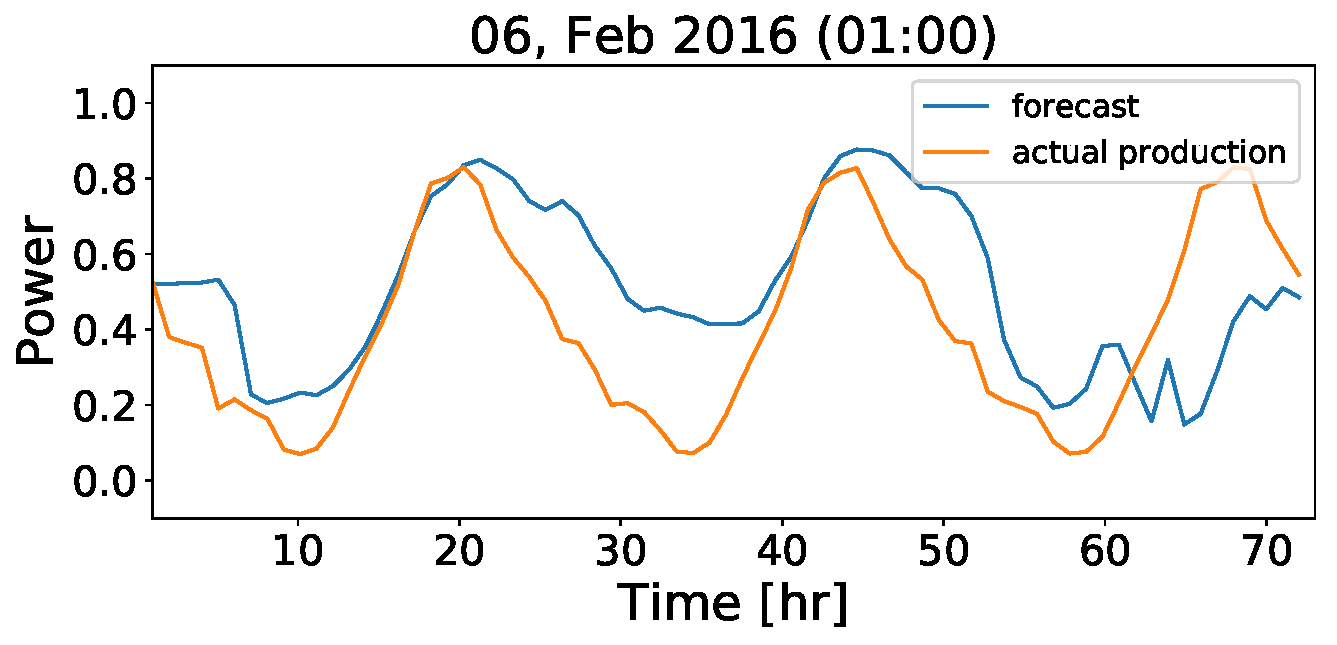
\includegraphics[width=1\linewidth]{Forecast_data_68.pdf}
    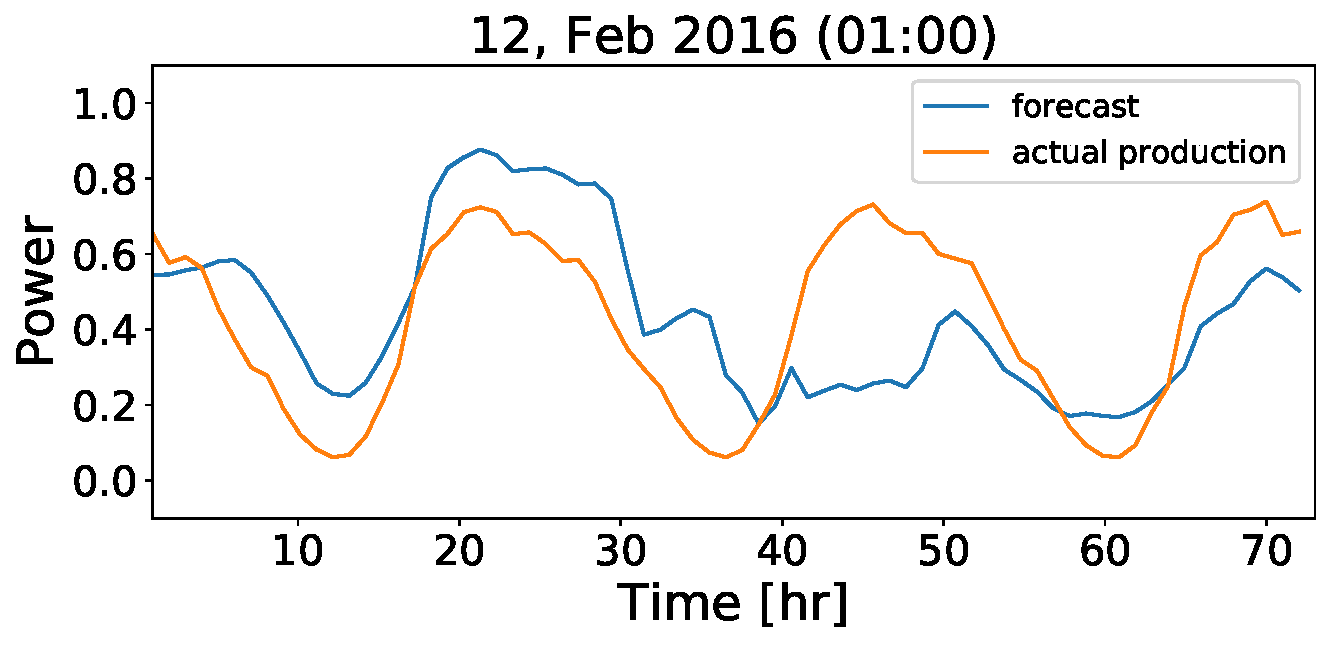
\includegraphics[width=1\linewidth]{Forecast_data_82.pdf}
\end{center}
   \caption{Examples of wind power generation set along with the wind power generation forecast from the data set.}
\label{fig:long}
\label{fig:onecol}
\end{figure}

\section*{Inference}
Using inference techniques, we were able to obtain the optimal parameters to our model of stochastic differential equations.\\

Moreover, the results are confirmed by the increasing accuracy of our optimal parameters estimation as we increase the number of samples in the data set.\\

The proposed model is computationally efficient, providing an accurate and reliable solution.


%\section*{Methodology}
%
%
%
%\begin{itemize}
%%\item The log-likelihood is convex in the  parameters $(\alpha, \theta_t )$ on the positive quadrant.
%\item We optimize using L-BFGS algorithm constrained to the positive quadrant.
%\end{itemize}
%The ellipse defined by the  Hessian of the log-likelihood shrinks at a fast rate as shown in Figure (\ref{ellipse_drawing}). The contours of the  log-likelihood can be seen in Figure (\ref{contour}).
%
%\begin{figure}[t]
%\begin{center}
%%\fbox{\rule{0pt}{2in} \rule{0.9\linewidth}{0pt}}
%    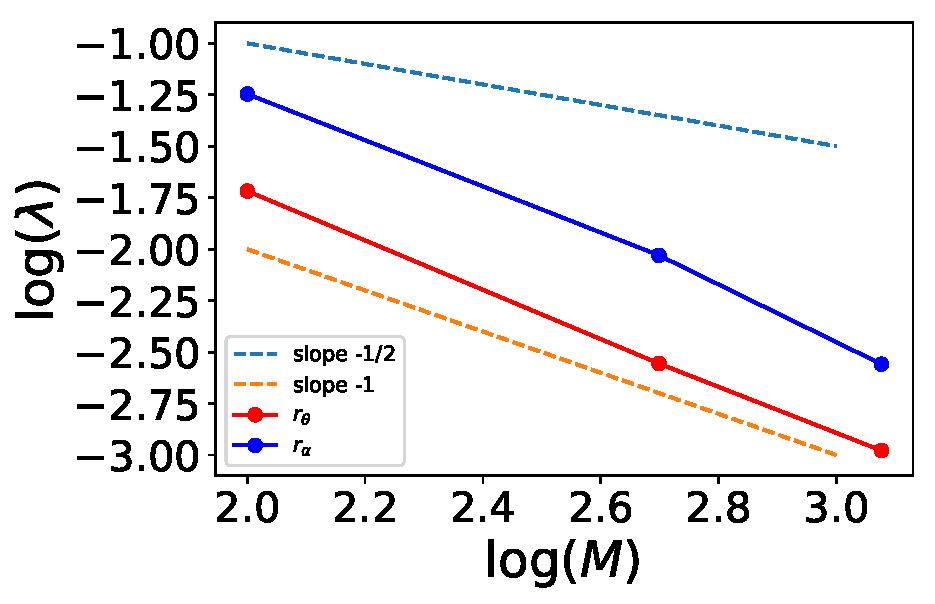
\includegraphics[width=0.6\linewidth]{ellipse_conv_samples_dN=14e-02.pdf}
%\end{center}
%   \caption{Left:Shrinkage of the ellipse determined by the Hessian matrix of the log-likelihood around the point of optimality $(\theta_0^*, \alpha^*)\approx (8,1)$ (Axis are not in natural scale, arrows only to  eignevector direction). Right: Convergence of the major and semi-axis of the ellipse  of the Hessian of the log-likelihood at the point optimality $(\theta_0^*, \alpha^*)\approx (8,1)$. Note that it is slightly faster than the expected rate of $1/\sqrt{M}$. This is due to the correlation structure of the process $V_t$, thus a path may act  as more than one  uncorrelated sample.}
%\label{ellipse_drawing}
%\end{figure}


% \quad\\
% \quad\\


\section*{Results}
 We were able to obtain the optimal  parameters of the model based on the complete data sets mentioned earlier.\\

 In Figure (\ref{simulated_24hr}) and (\ref{simulated_12hr}), we simulate possible  paths wind power production for a given wind power forecast.

 %Note that the confidence bands obtained are non-trivial and reflect the complexity of the uncertainties in numerical wind power generation forecasts.

 \begin{figure}[t]
 \begin{center}
 %\fbox{\rule{0pt}{2in} \rule{0.9\linewidth}{0pt}}
    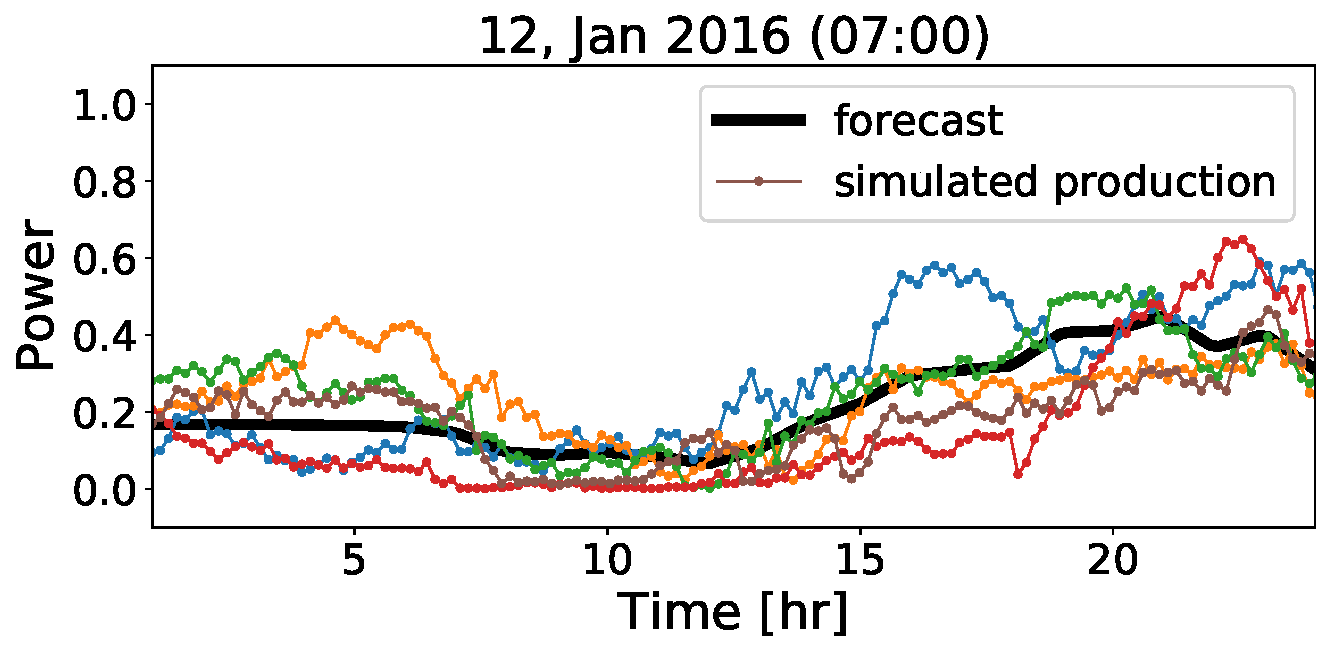
\includegraphics[width=1\linewidth]{simulated/24hr/19.pdf}  %569
    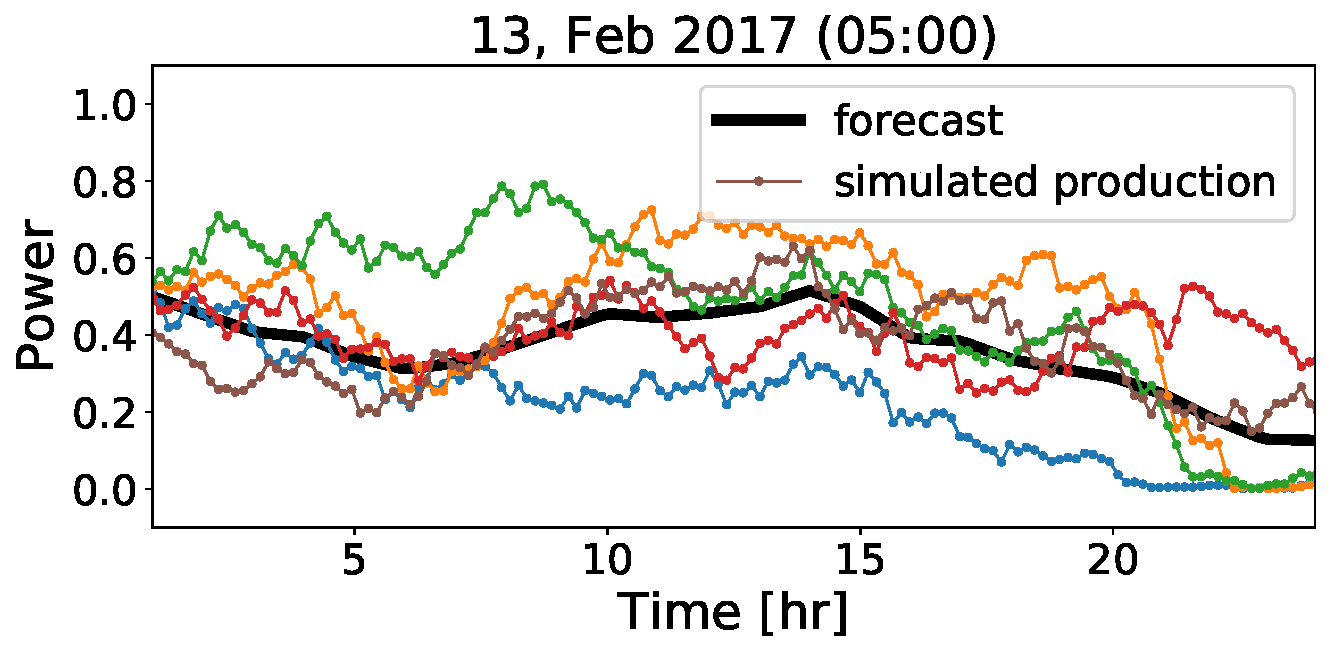
\includegraphics[width=1\linewidth]{simulated/24hr/1099.pdf}
    %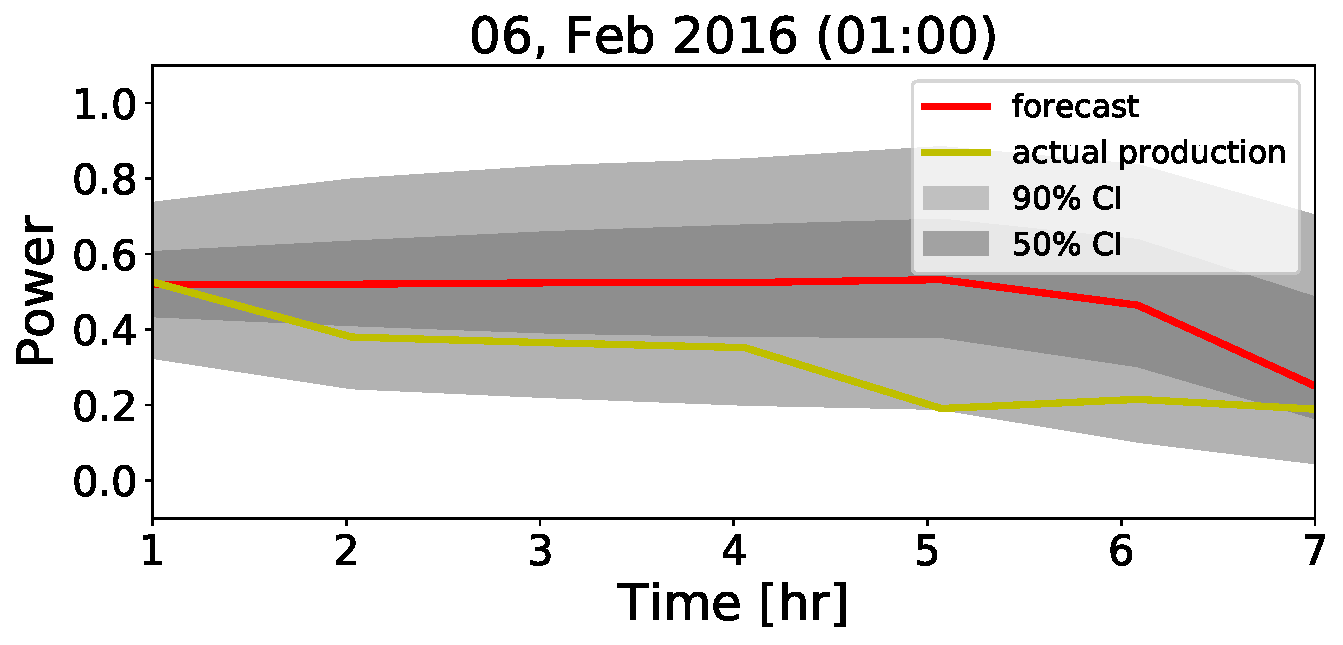
\includegraphics[width=0.9\linewidth]{6hr_forecast_CI_68.pdf}
 \end{center}
    \caption{ Examples of simulated paths of wind power production for the next 24 hours.}
 \label{simulated_24hr}
 \end{figure}

 \begin{figure}[t]
 \begin{center}
 %\fbox{\rule{0pt}{2in} \rule{0.9\linewidth}{0pt}}
    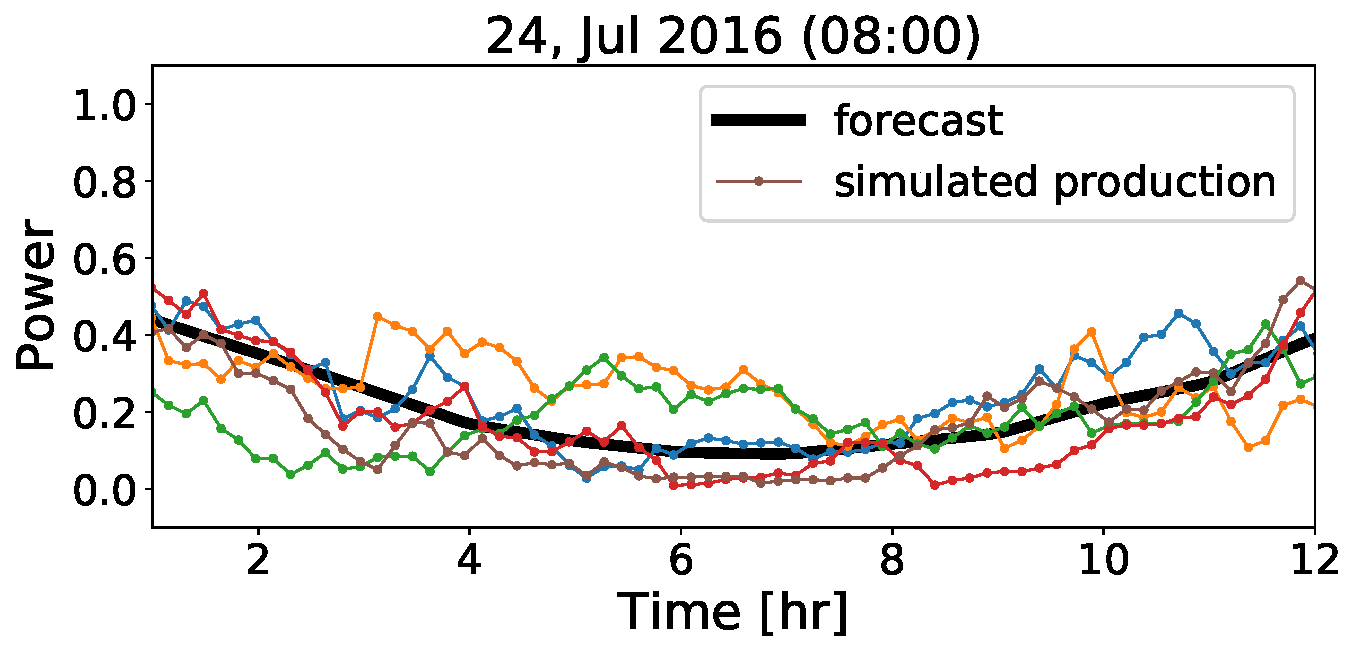
\includegraphics[width=1\linewidth]{simulated/12hr/622.pdf}  %569
    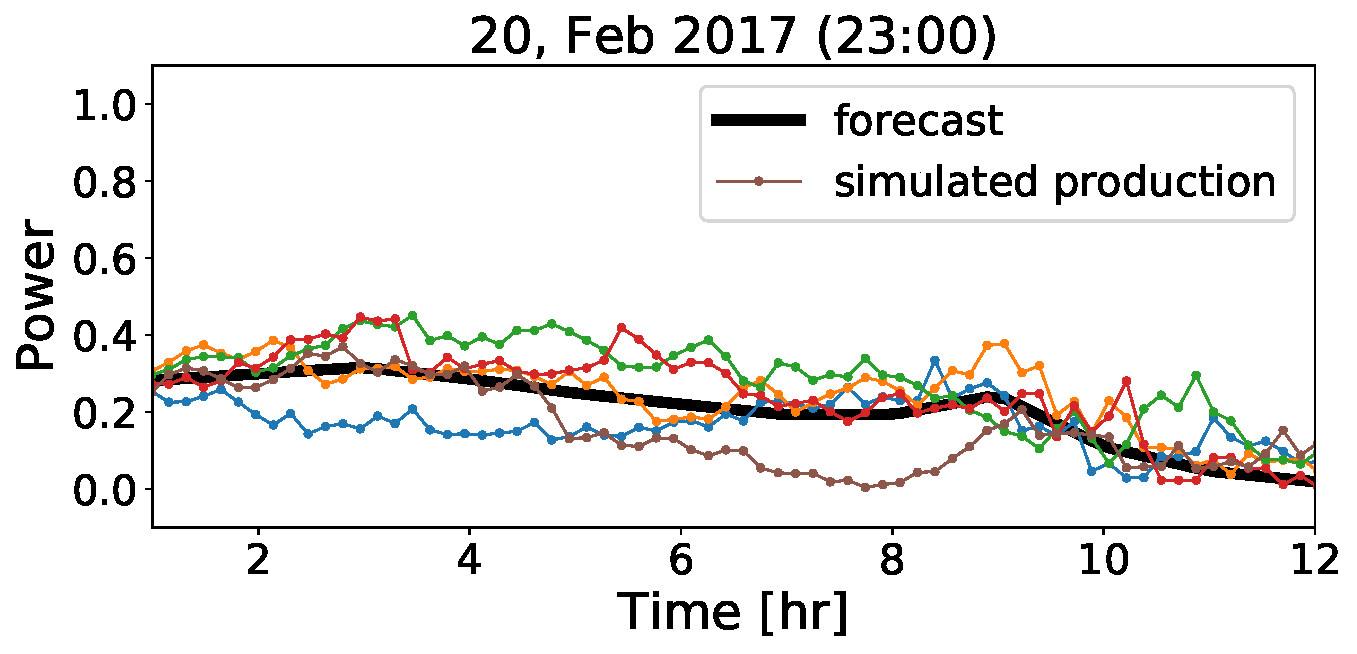
\includegraphics[width=1\linewidth]{simulated/12hr/1124.pdf}
    %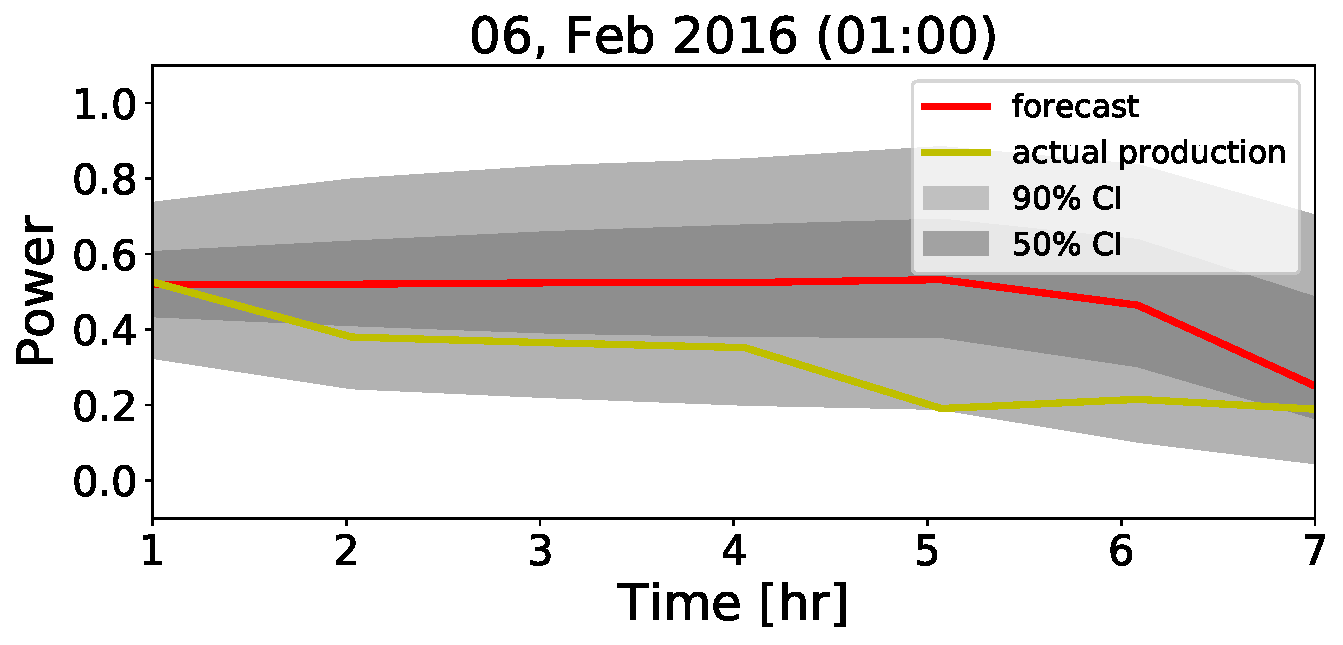
\includegraphics[width=0.9\linewidth]{6hr_forecast_CI_68.pdf}
 \end{center}
    \caption{ Examples of simulated paths of wind power production for the next 12 hours.}
 \label{simulated_12hr}
 \end{figure}

 In Figure (\ref{fig:72hr}) and (\ref{fig:6hr}), we obtain empirical confidence bands using the optimal parameters.

\begin{figure}[t]
\begin{center}
%\fbox{\rule{0pt}{2in} \rule{0.9\linewidth}{0pt}}
   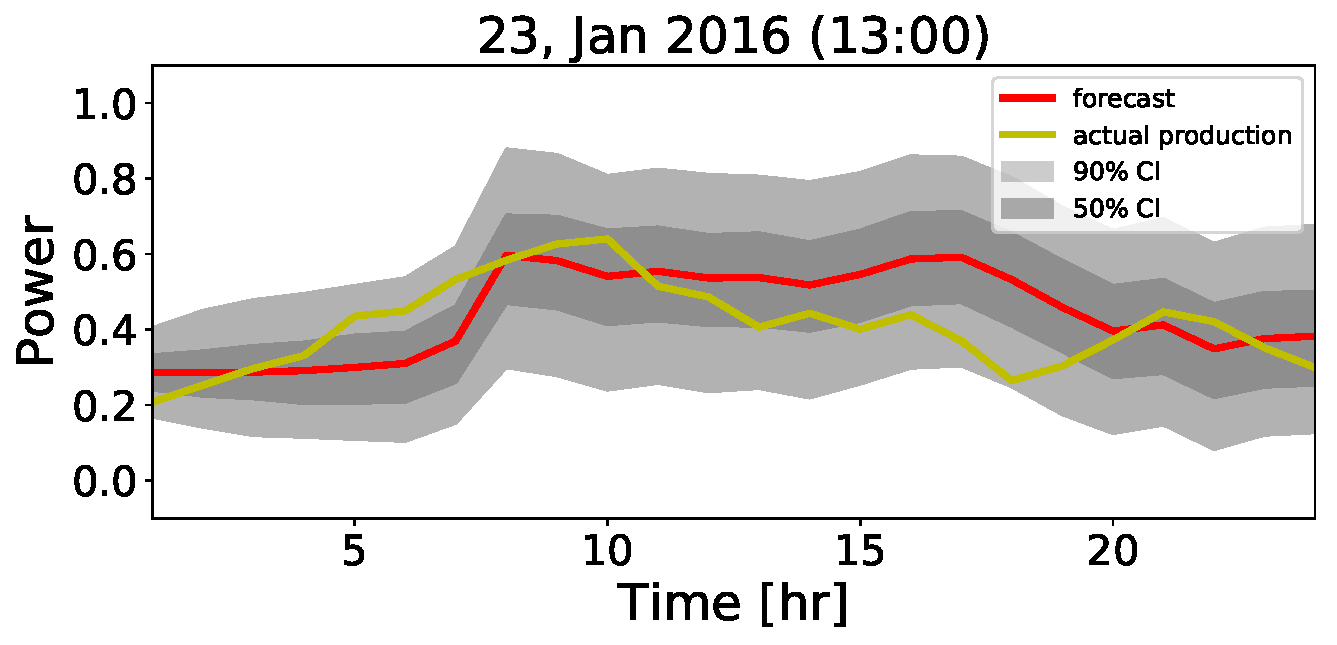
\includegraphics[width=1\linewidth]{confidence_intervals/24hr/31.pdf}
   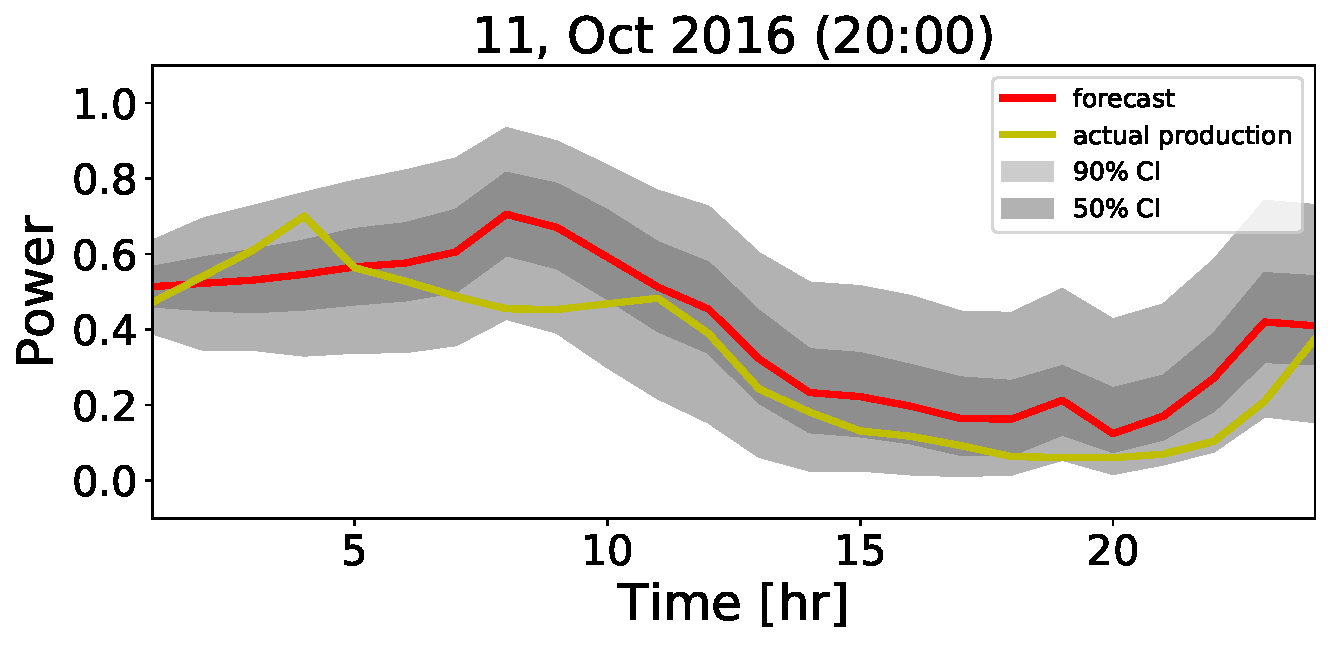
\includegraphics[width=1\linewidth]{confidence_intervals/24hr/820.pdf}
   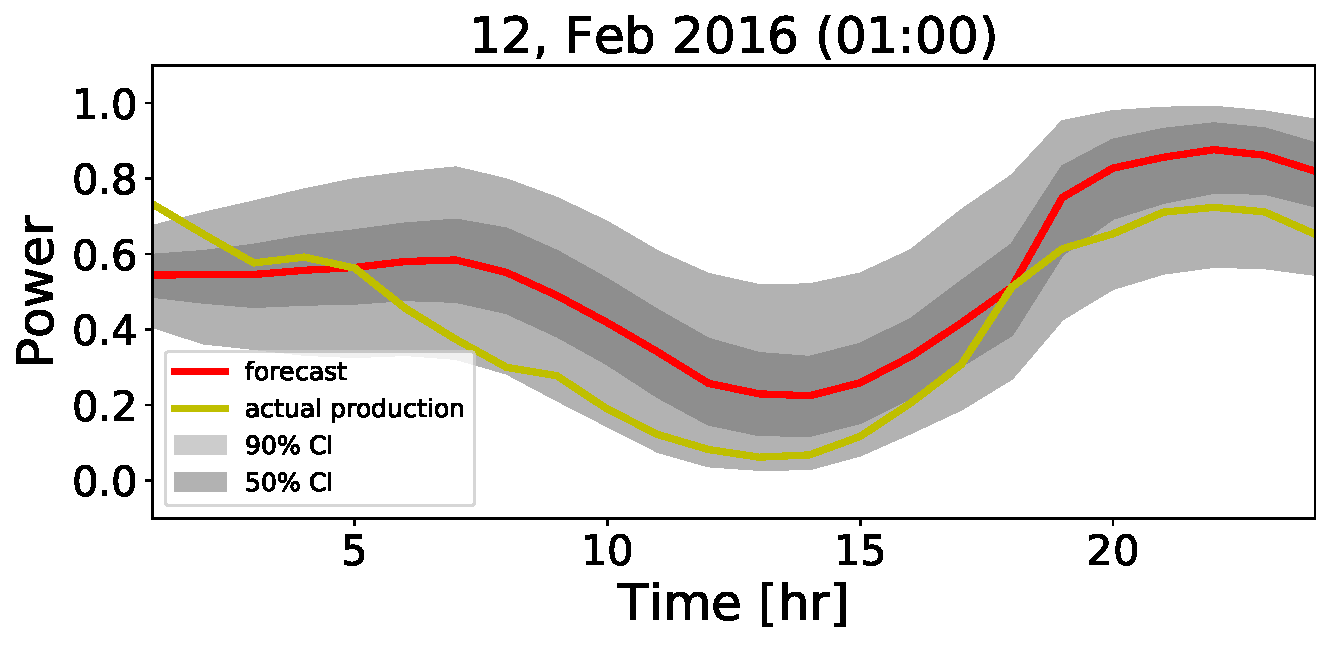
\includegraphics[width=1\linewidth]{confidence_intervals/24hr/82.pdf}

\end{center}
   \caption{ Examples of confidence bands obtained for 24 hour forecasts. We can see that the model captures the fluctuations in the actual production with non-trivial and asymmetric confidence intervals.}
\label{fig:72hr}
\end{figure}

\begin{figure}[t]
\begin{center}
%\fbox{\rule{0pt}{2in} \rule{0.9\linewidth}{0pt}}
   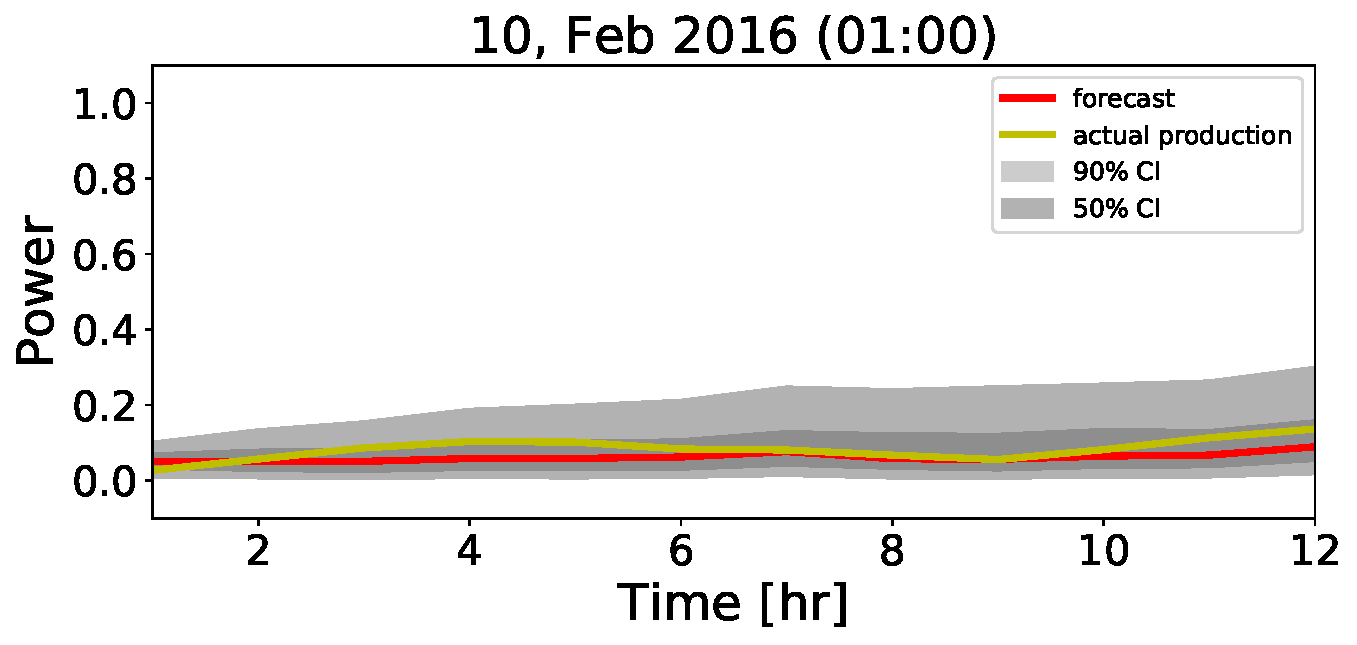
\includegraphics[width=1\linewidth]{confidence_intervals/12hr/75.pdf}
   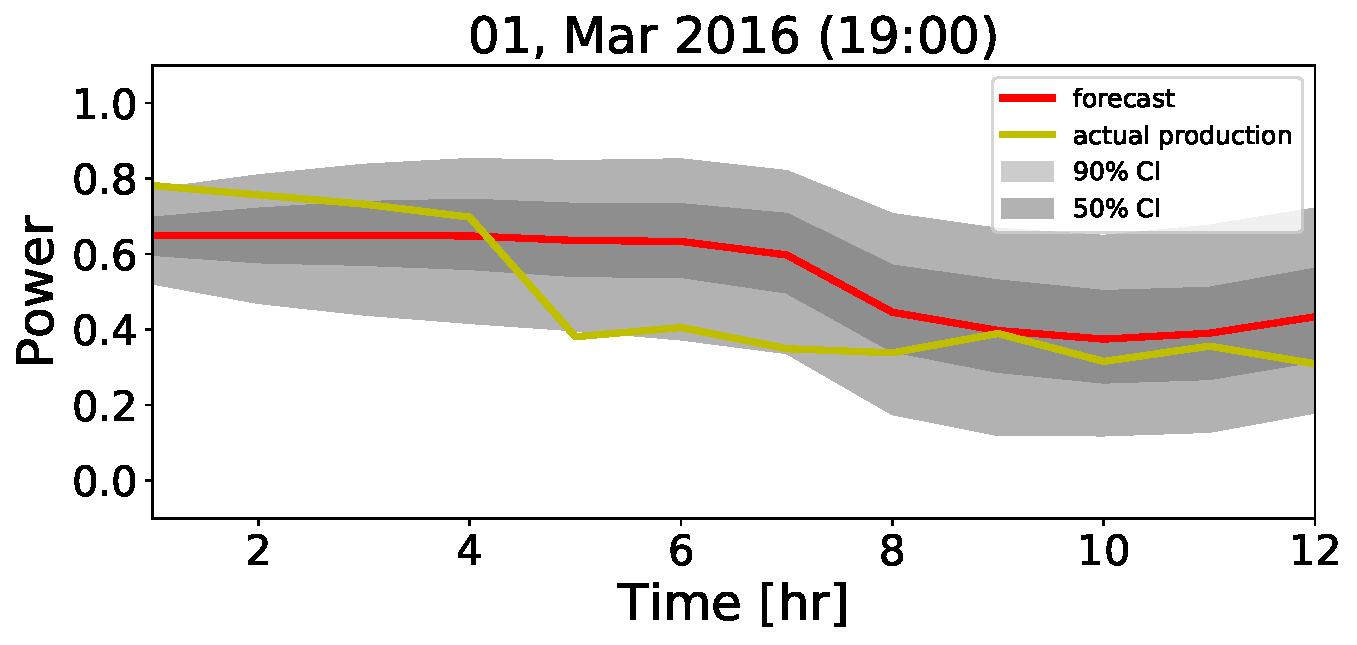
\includegraphics[width=1\linewidth]{confidence_intervals/12hr/148.pdf}
   %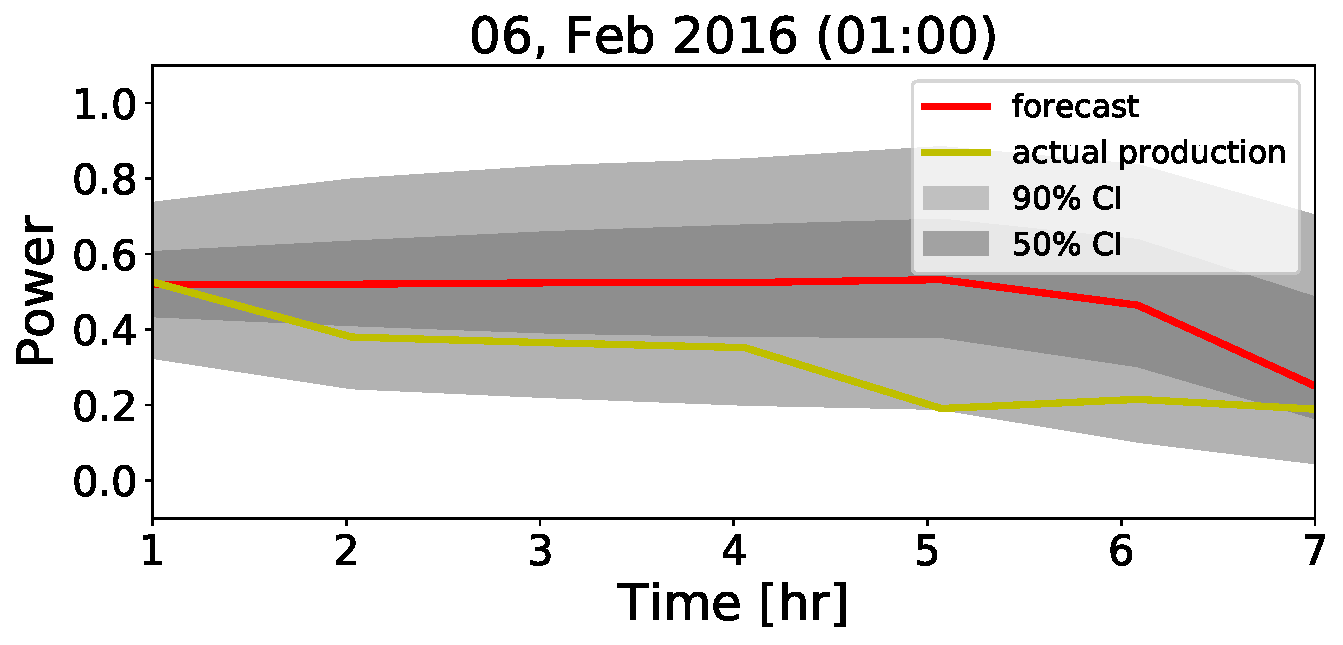
\includegraphics[width=0.9\linewidth]{6hr_forecast_CI_68.pdf}
\end{center}
   \caption{ Examples of confidence bands obtained for the first 12 hours of the forecasts. Note that this forecasting company computes a new forecast every 6-9 hours for reliability.}
\label{fig:6hr}
\end{figure}


% \begin{figure}[t]
%\begin{center}
%%\fbox{\rule{0pt}{2in} \rule{0.9\linewidth}{0pt}}
%   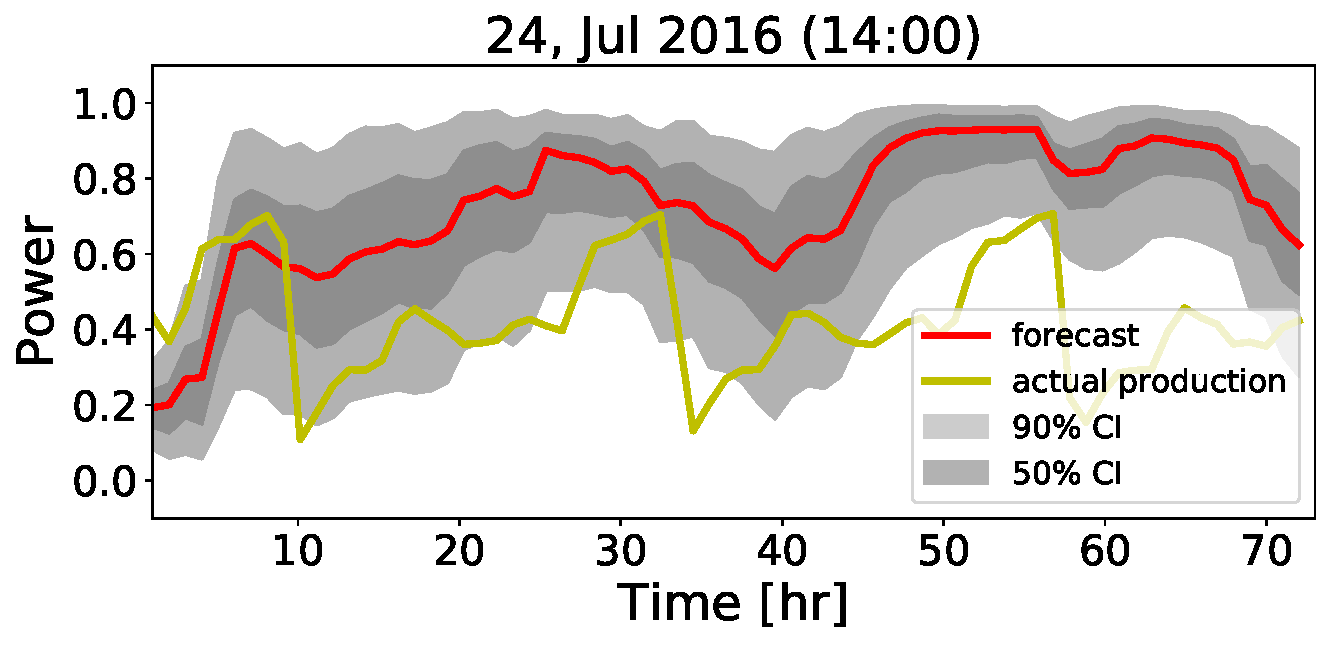
\includegraphics[width=0.8\linewidth]{72hr_forecast_CI_623.pdf}  %569
%\end{center}
%   \caption{ Examples of omitted data which corresponds to production control and manual energy management decisions. In this example,  wind power production was repeatedly curtailed at around 2 AM which is a period of low power demand. Automatic detection of such scenarios is to be incorporated in future works.}
%\label{fig:6hr}
%\end{figure}

\section*{Conclusions}
In this project, we have proposed a model based on parametric Stochastic Differential Equations and advanced inference to quantify uncertainties in wind power generation forecasts. It has the following advantages:
\begin{itemize}
\item  Represents and quantifies uncertainty in wind power forecasts accordingly to their real-world performance.
\item Ability to simulate paths of wind power production.
\item It is forecast technology agnostic.
\item  Takes into account physical constrains and the skew-symmetric nature of forecast error.
\item Provides a basis for decision making in the optimal dispatch of electric power.
\end{itemize}

%\section*{Acknowledgement}

% \section*{References}
% \begin{flushleft}
% [1] {Elkantassi, S., Kalligiannaki, E., \& Tempone, R. (2017). Inference And Sensitivity In Stochastic Wind Power Forecast Models. Proceedings of the 2nd International Conference on Uncertainty Quantification in Computational Sciences and Engineering (UNCECOMP 2017). doi:10.7712/120217.5377.16899}
% \end{flushleft}

\end{multicols}
\end{document}
